Als Ladungsverstärker bezeichnet man elektrische Schaltungen welche ein Spannungssignal proportional zu einer bestimmten Ladung erzeugen.
Diese Art von Schaltung wird häufig als Ausleseelektronik für Ionisationskanäle verwendet da bei einem Event eine bestimmte Anzahl Ladung in Form von Elektron-Loch-Paaren entsteht.
Die Anzahl der Elektron-Loch-Paare ist wiederum proportional zur deponierten Energie des Events.
Bei Germanium Kristallen, wie sie bei DeLight und CDMS verwedet werden, entsteht ein Elektron-Loch-Paar pro $\sim\SI{3}{\electronvolt}$ deponierter Energie.

In Abbildung \ref{fig:Ladungsverstärker} ist die grundlegende Struktur eines Ladungsverstärkers dargestellt.
Der Detektor wird entsprechend dem Ramo-Theorem im Ersatzschaltbild durch eine Stromquelle parallel zur Detektorkapazität dargestellt.
Der Signalstrom ist nach Gleichung \eqref{eq:RamoCurrent} abhängig von der Driftgeschwindigkeit.
In Germanium beträgt diese mehrere $\SI{}{\centi\meter}/\SI{}{\micro\second}$.
Um in einem $\sim\SI{2}{\centi\meter}$ dicken Detektor den genauen Stromverlauf zu verfolgen ist somit ein Verstärker mit einer Bandbreite von mehreren $\SI{}{\mega\hertz}$ notwendig.
Aufgrund der großen Detektorkapazität und den langen Kabeln zwischen Detektor und Ausleseelektronik ist die Bandbreite von Ladungsverstärkern in der Regel auf mehrere hundert $\SI{}{\kilo\hertz}$ begrenzt.
Daher kann der Signalstrom als Deltapeak modelliert werden.
\begin{equation}
i_{sig} = \Delta Q \delta(t)
\end{equation}

\begin{figure}[!t]
\begin{center}
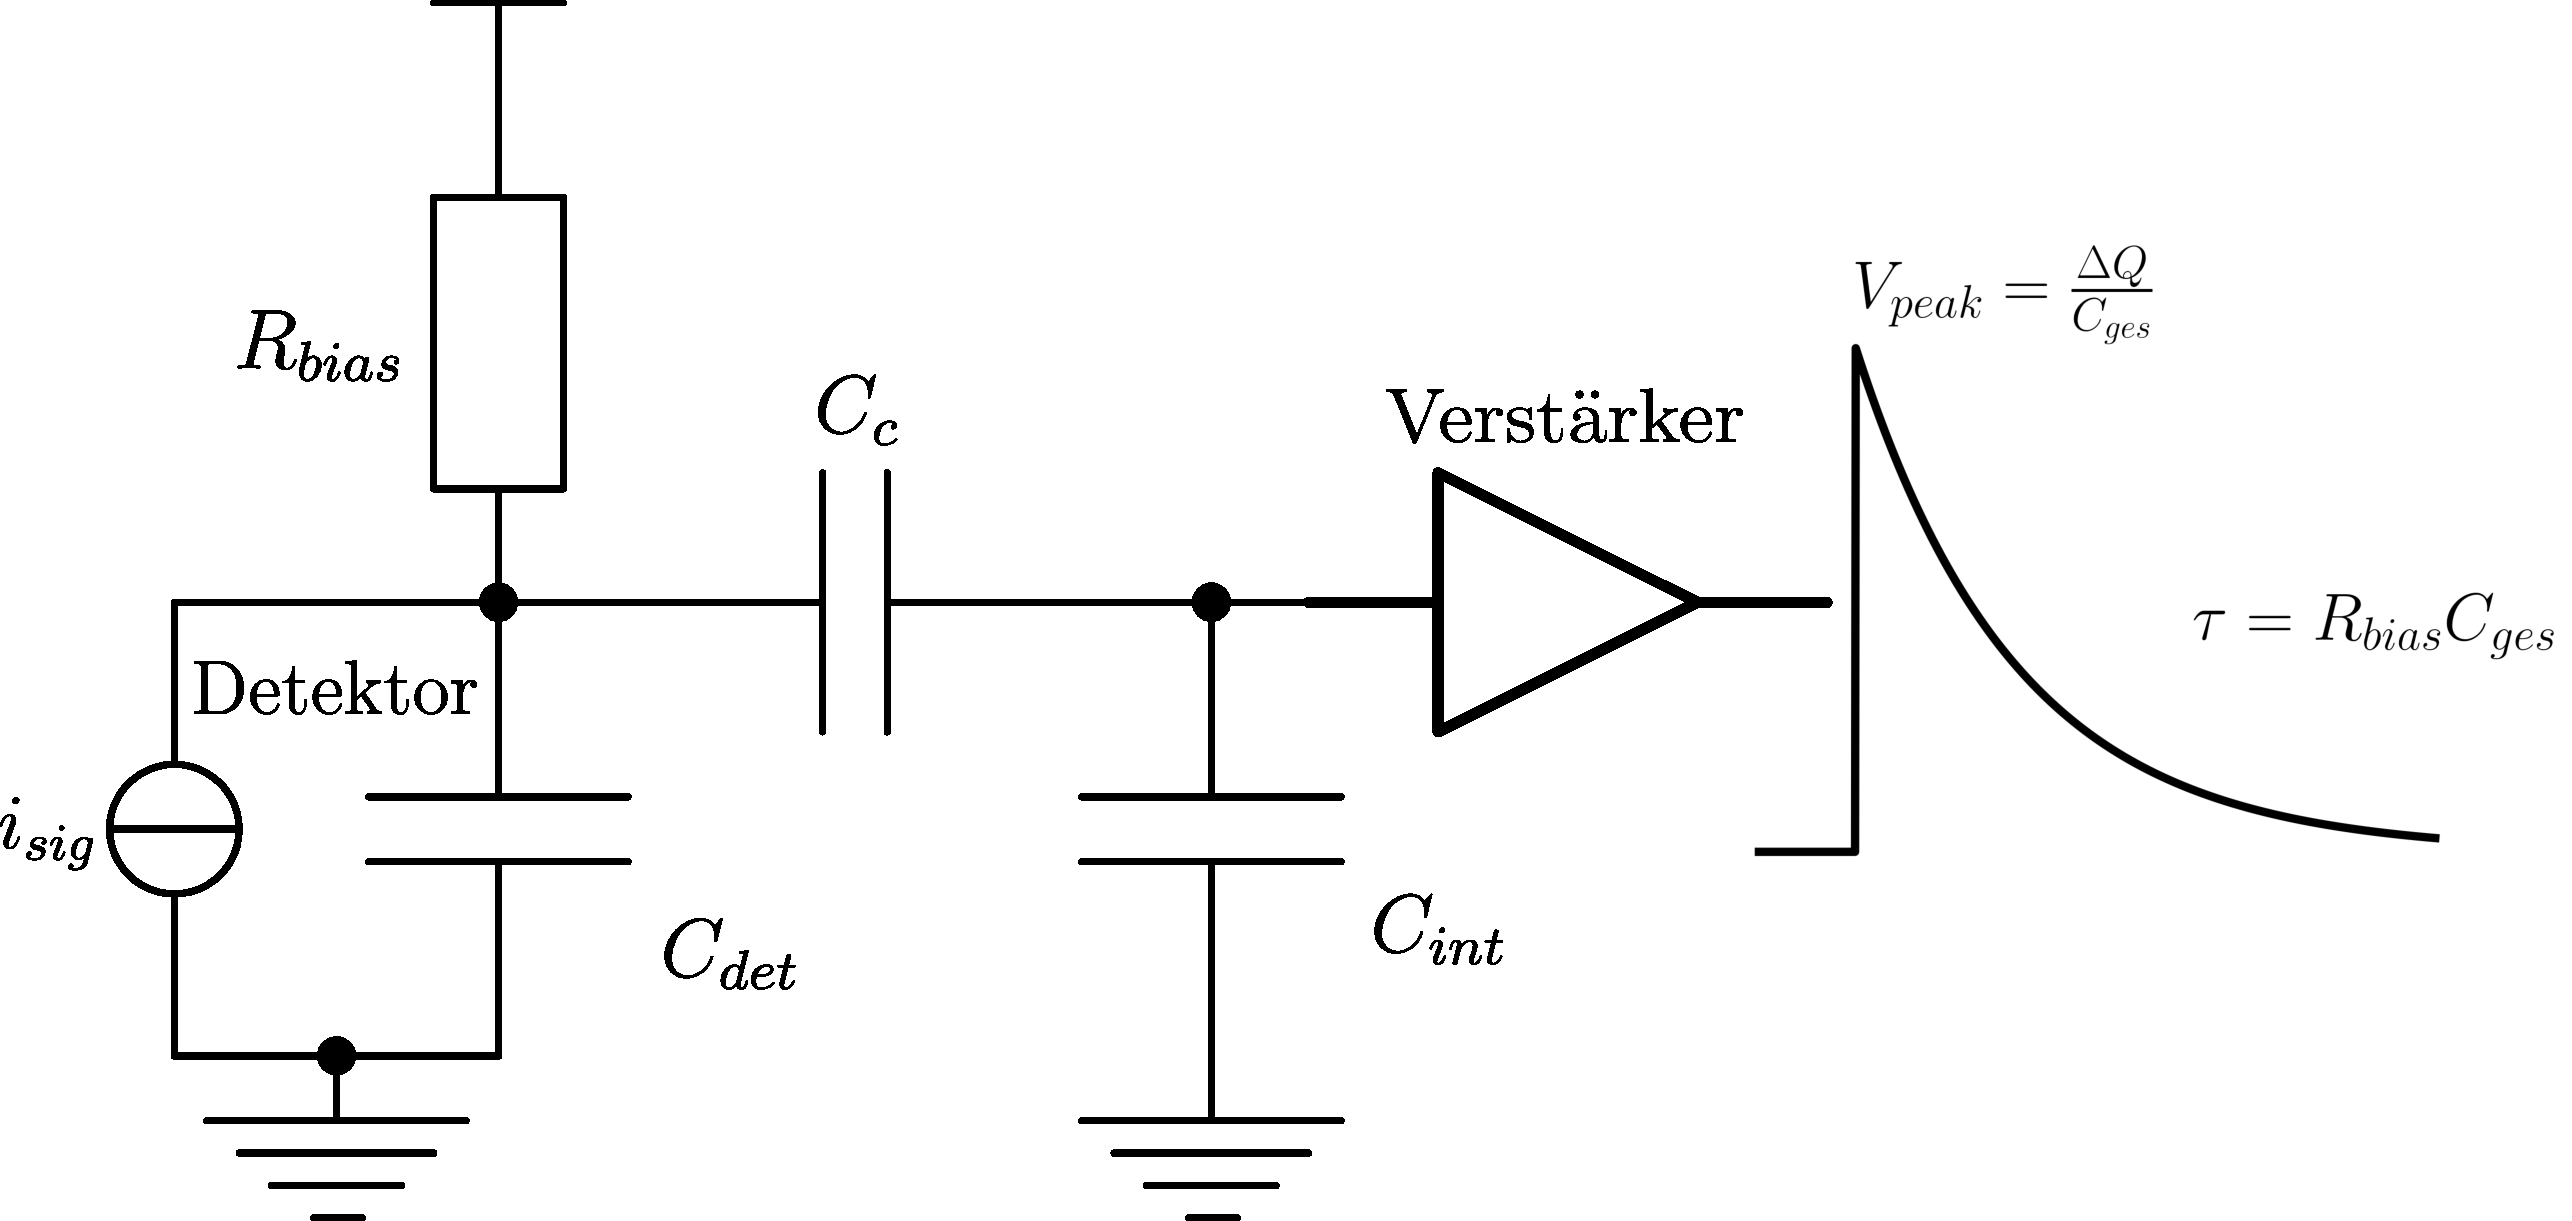
\includegraphics[scale=0.35]{./fig/Ladungsverstaerker.pdf}
\vspace{-0.5cm}
\caption{Grundlegende Schaltung eines Ladungsverstärkers.}
\label{fig:Ladungsverstärker}
\end{center}
\end{figure}

Über den Biaswiderstand $R_{bias}$ wir der Detektor gespannt ohne dass der Signalstrom kurz geschlossen wird.
Der Biaswiderstand wird in der Regel groß gewählt sodass es nicht zur Entladung kommt bevor der Signalpeak seine maximale höhe Erreicht.
Des weiteren bedeutet ein großer Biaswiderstand kleineres Wärmerauschen.

Die Koppelkapazität $C_c$ erlaubt es unterschiedliche DC Level am Detektor und am Verstärkereingang anzulegen.
Am Detektor sollen Spannungen in der Größenordnung $\mathcal{O}(\SI{100}{\volt})$ anliegen.
und am Verstärkereingang $\mathcal{O}(\SI{-100}{\milli\volt})$.
Das heißt die Kapazität $C_c$ muss für große Spannungsdifferenzen ausgelegt sein.

Die Kapazität $C_{int}$ integriert am Verstärkereingang den Signalstrom.
Damit an der Koppelkapazität keine Spannung abfällt muss diese deutlich größer sein als die Kapazität $C_{int}$.

Um die genaue Signalform zu bestimmten ist es sinnvoll in den Frequenzraum zu wechseln.
Dort ist der Signalstrom durch $i_{sig}(f)=\Delta Q$ gegeben.
Dann gilt für das Spannungsignal
\begin{align*}
V(f) &= i_{sig}(f)Z_{in} \nonumber \\
&= \Delta Q Z_{R_{bias}}||Z_{C_{ges}} \nonumber \\
&= \Delta Q \frac{R_{bias}}{1 + i2\pi f C_{ges} R_{bias}}.
\end{align*}
Durch Rücktransformation erhalten wir
\begin{align*}
V(t) &= \frac{\Delta Q}{C_{ges}}\Theta(t)e^{-\frac{t}{\tau}} \nonumber \\
&\stackrel{\eqref{eq:RamoCharge}}{=} \frac{-eN_{eh}(a-b)}{C_{ges}}\Theta(t)e^{-\frac{t}{\tau}}
\end{align*}
mit der Zeitkonstante $\tau=C_{ges}R_{bias}$ und der Heaviside-Sprungfunktion $\Theta(t)$.


